% ============================================================
%  第 2 章  复变函数论（扩展版）
% ============================================================

\chapter{复变函数论}

\section{本章概览与学习路线}

复变函数是本科物理数学工具中"性价比"最高的一个分支——它需要的预备知识最少（只需要微积分和一阶线性代数），但带来的收益巨大：交流电路分析、二维场论、量子力学、色散关系、信号处理，无一不依赖复变函数。

\begin{center}
\fbox{\parbox{0.9\textwidth}{\centering
\textbf{核心逻辑链条：}\\
复数代数 $\to$ 解析函数（C-R 方程）$\to$ 复积分（Cauchy 理论）$\to$ 留数定理 $\to$ 物理应用
}}
\end{center}

\subsection*{不同读者的学习路径}

\begin{itemize}
\item \textbf{物理专业学生：} 重点关注 \S2.2（相量法）、\S2.6（留数定理算实积分）、\S2.7（保角映射与二维场）、\S2.8（Kramers-Kronig 关系）。\S2.4（多值函数）在初步阅读时只需理解基本概念。
\item \textbf{数学/应用数学学生：} 重点关注 \S2.3--\S2.6 的严格推导和证明，特别是 Cauchy 理论、留数定理的完整证明、多值函数的 Riemann 曲面解释。
\item \textbf{电子工程学生：} 重点关注 \S2.2（相量法和复阻抗）、\S2.6（留数定理）、\S2.7（保角映射在传输线中的应用）。
\end{itemize}

\section{复数与相量法}
\label{sec:complex_basics}

\subsection*{动机：为什么物理学家喜欢复数？}

没有复数，交流电路中的每个 $RLC$ 问题都需要解一个二阶微分方程。有了复数，$L$ 的 $v_L = L\,\dd i/\dd t$ 变成 $\tilde{V}_L = \mathrm{i}\omega L\,\tilde{I}$——微分变成了乘法！这是线性系统分析中的第一次"换域操作"：从时域到频域。你后面会遇到类似的域变换：傅里叶变换、拉普拉斯变换。复数就是这一思想的起点。

\subsection{复数的表示}

\textbf{代数形式：} $z = x + \mathrm{i}y$，其中 $x=\Re(z)$, $y=\Im(z)$。

复数可以看作二维平面上的点 $(x,y)$。加法就是向量加法，乘法则引入了全新的结构——旋转和缩放。

\textbf{极坐标形式：}
\begin{equation}
z = r(\cos\theta + \mathrm{i}\sin\theta) = re^{\mathrm{i}\theta},
\qquad r = |z| = \sqrt{x^2+y^2},\;
\theta = \arg z.
\end{equation}

这里 $r = |z|$ 是模长，$\theta = \arg z$ 是辐角。辐角不是唯一的——$\theta + 2\pi k$ 都对应同一个复数。在后面我们会看到，这种"多值性"有深刻的物理后果。

\textbf{欧拉公式}（数学中最优美的公式之一）：
\begin{equation}
e^{\mathrm{i}\theta} = \cos\theta + \mathrm{i}\sin\theta.
\label{eq:euler}
\end{equation}

$\theta = \pi$ 给出 $e^{\mathrm{i}\pi} + 1 = 0$，将五个最重要的数学常数联系在了一起：$e$、$\mathrm{i}$、$\pi$、$1$、$0$。

% 复平面图
\begin{figure}[H]
\centering
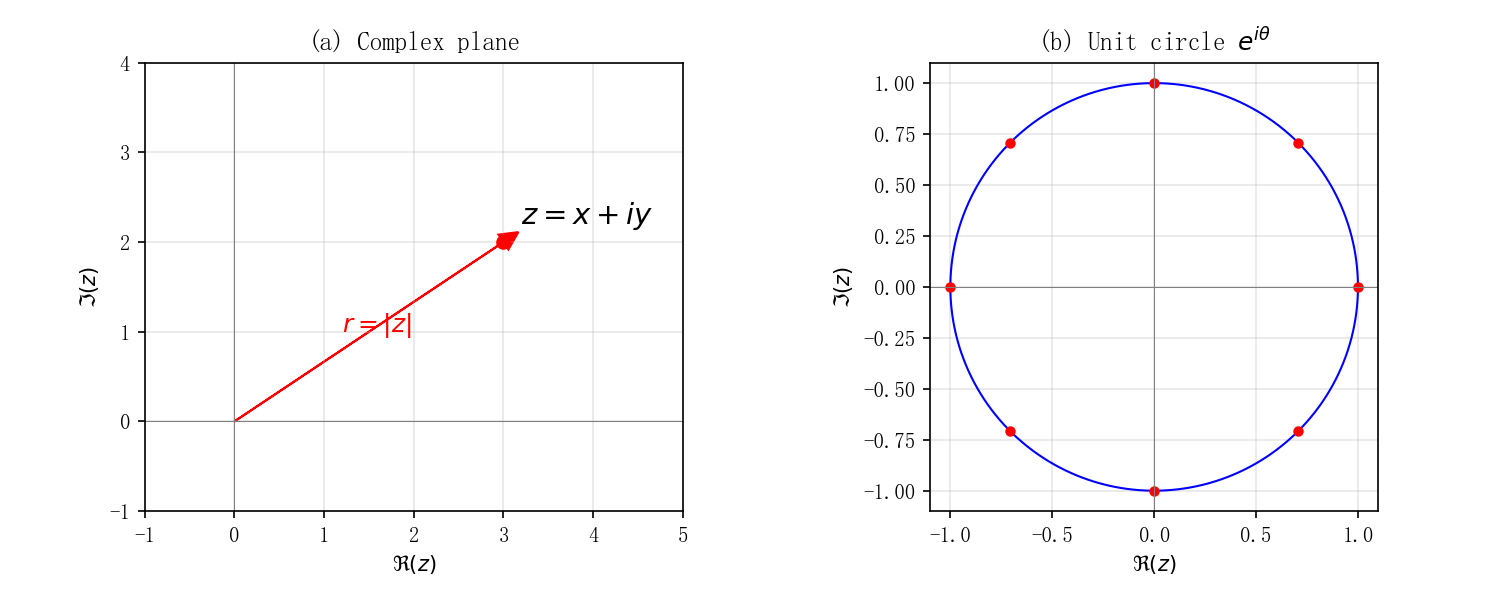
\includegraphics[width=0.75\textwidth]{figures/fig2_1_complex_plane.png}
\caption{左：复平面中 $z=x+iy$ 的矢量表示。右：单位圆 $e^{i\theta}$ 上的 8 个等分点。注意旋转 $\pi/4$ 对应乘以 $e^{i\pi/4}$。}
\label{fig:complex_plane}
\end{figure}

\subsection{复数的代数运算}

设 $z_1 = x_1 + \mathrm{i}y_1$, $z_2 = x_2 + \mathrm{i}y_2$：

\begin{align*}
\text{加法：}\quad &z_1 + z_2 = (x_1+x_2) + \mathrm{i}(y_1+y_2),\\
\text{乘法：}\quad &z_1 z_2 = (x_1 x_2 - y_1 y_2) + \mathrm{i}(x_1 y_2 + x_2 y_1),\\
\text{共轭：}\quad &\bar{z} = x - \mathrm{i}y,\quad z\bar{z} = |z|^2 = x^2 + y^2,\\
\text{除法：}\quad &\frac{z_1}{z_2} = \frac{z_1\bar{z_2}}{|z_2|^2} = \frac{(x_1 x_2 + y_1 y_2) + \mathrm{i}(x_2 y_1 - x_1 y_2)}{x_2^2 + y_2^2}.
\end{align*}

乘法的极坐标形式尤为优雅：$z_1 z_2 = r_1 r_2 e^{\mathrm{i}(\theta_1 + \theta_2)}$——模长相乘，辐角相加。这意味着乘法 = 旋转 + 缩放。

\begin{example}[复数的基本运算]
设 $z_1 = 1 + 2\mathrm{i}$, $z_2 = 3 - \mathrm{i}$。计算：

\textbf{(1)} $z_1 + z_2 = (1+3) + \mathrm{i}(2-1) = 4 + \mathrm{i}$。

\textbf{(2)} $z_1 z_2 = (1\cdot3 - 2\cdot(-1)) + \mathrm{i}(1\cdot(-1) + 2\cdot3) = (3+2) + \mathrm{i}(-1+6) = 5 + 5\mathrm{i}$。

用极坐标验证：$z_1 = \sqrt{5}e^{\mathrm{i}\arctan 2}$, $z_2 = \sqrt{10}e^{-\mathrm{i}\arctan(1/3)}$，乘积的模为 $\sqrt{50}=5\sqrt{2}$，辐角为 $\arctan 2 - \arctan(1/3) = \arctan(1)$（可以验证），所以确实 $5 + 5\mathrm{i}=5\sqrt{2}e^{\mathrm{i}\pi/4}$。

\textbf{(3)} $1/z_1 = \frac{1-2\mathrm{i}}{1^2+2^2} = \frac{1}{5} - \frac{2}{5}\mathrm{i}$。

\textbf{(4)} $|z_1| = \sqrt{1^2+2^2} = \sqrt{5}$, $|\bar{z}_1| = \sqrt{5}$, $\overline{z_1+z_2} = 4 - \mathrm{i}$。
\end{example}

\begin{insight}[相量法的物理核心]
交流电路中的正弦激励 $V(t) = V_0\cos(\omega t + \phi)$ 可以看作复相量 $V_0 e^{\mathrm{i}(\omega t+\phi)}$ 的实部。微分和积分运算变为：
\begin{align}
\frac{\dd}{\dd t} e^{\mathrm{i}\omega t} &= \mathrm{i}\omega e^{\mathrm{i}\omega t},\\
\int e^{\mathrm{i}\omega t}\,\dd t &= \frac{1}{\mathrm{i}\omega} e^{\mathrm{i}\omega t}.
\end{align}
于是 $RLC$ 串联电路的微分方程
\begin{equation}
L\frac{\dd I}{\dd t} + RI + \frac{1}{C}\int I\,\dd t = V(t)
\end{equation}
变为复数代数方程
\begin{equation}
\left(\mathrm{i}\omega L + R + \frac{1}{\mathrm{i}\omega C}\right)\tilde{I} = \tilde{V},
\end{equation}
其中括号内正是复阻抗 $Z$。这就是相量法——将时域微积分转化为频域代数运算，极大简化了线性电路分析。
\end{insight}

\subsection{复数的几何意义}

复数的乘法有重要的几何解释：

\begin{itemize}
\item 乘以 $re^{\mathrm{i}\theta}$ = 缩放 $r$ 倍 + 逆时针旋转 $\theta$ 角。
\item 乘以 $\mathrm{i}$ = 逆时针旋转 $90^\circ$（因为 $\mathrm{i} = e^{\mathrm{i}\pi/2}$）。
\item 乘以 $-1$ = 旋转 $180^\circ$。
\end{itemize}

\begin{example}[几何意义的可视化]
在复平面上画出下列变换：

\textbf{(1)} $z \to \mathrm{i}z$：点 $(x,y)$ 被映射到 $(-y,x)$，即绕原点逆时针旋转 $90^\circ$。

\textbf{(2)} $z \to z^2$：模变为平方，辐角加倍。单位圆上的点 $e^{\mathrm{i}\theta}$ 变为 $e^{2\mathrm{i}\theta}$——这意味着单位圆上的点被"拉伸"到两倍角速度。它在物理中的一个应用是倍频器。

\textbf{(3)} $z \to 1/z$：模取倒数，辐角变号。这是反演变换，将单位圆内的点映射到外部，反之亦然。
\end{example}

\subsection{复数的乘幂与单位根}

棣莫弗公式：
\begin{equation}
(re^{\mathrm{i}\theta})^n = r^n e^{\mathrm{i}n\theta},
\quad
z^{1/n} = r^{1/n} e^{\mathrm{i}(\theta+2\pi k)/n},\; k=0,1,\dots,n-1.
\end{equation}

单位根 $z^n = 1$ 的 $n$ 个解均匀分布在单位圆上：
\begin{equation}
\omega_k = e^{2\pi\mathrm{i}k/n},\quad k=0,1,\dots,n-1.
\end{equation}

\begin{example}[完整算例：三次单位根]
求 $z^3 = 1$ 的所有解。
\begin{align*}
z_0 &= e^{0} = 1,\\
z_1 &= e^{2\pi\mathrm{i}/3} = -\frac12 + \mathrm{i}\frac{\sqrt3}{2},\\
z_2 &= e^{4\pi\mathrm{i}/3} = -\frac12 - \mathrm{i}\frac{\sqrt3}{2}.
\end{align*}
三个解在复平面上构成等边三角形。验证：$1 + z_1 + z_2 = 0$。
\end{example}

\begin{example}[四次单位根与离散傅里叶变换]
$z^4 = 1$ 的四个解为 $1,\mathrm{i},-1,-\mathrm{i}$。将它们记为 $\omega_0=1,\omega_1=\mathrm{i},\omega_2=-1,\omega_3=-\mathrm{i}$。

这四个根构成了 $4\times4$ 傅里叶矩阵的基础：
\begin{equation}
F_{jk} = \frac{1}{\sqrt{4}}\omega_4^{-jk},\quad j,k=0,1,2,3.
\end{equation}
这是 DFT（离散傅里叶变换）在 $N=4$ 时的特例，将在第 3 章中详细讨论。
\end{example}

\subsection{复数的物理应用：交流电路中的复阻抗}

\begin{example}[完整算例：RC 电路的低通滤波特性]
考虑一个串联 RC 电路，电阻 $R$，电容 $C$，输入电压 $V_{\text{in}}(t) = V_0\cos(\omega t)$。

\textbf{步骤 1：写出复阻抗。}
$Z_R = R$, $Z_C = 1/(\mathrm{i}\omega C) = -\mathrm{i}/(\omega C)$。
总阻抗 $Z = R + 1/(\mathrm{i}\omega C) = R - \mathrm{i}/(\omega C)$。

\textbf{步骤 2：计算复电流。}
$\tilde{I} = \frac{\tilde{V}_{\text{in}}}{Z} = \frac{V_0}{R - \mathrm{i}/(\omega C)}$。

\textbf{步骤 3：输出电压（电容两端）。}
\begin{align*}
\tilde{V}_{\text{out}} &= \tilde{I} \cdot \frac{1}{\mathrm{i}\omega C}
= V_0 \frac{1/(\mathrm{i}\omega C)}{R + 1/(\mathrm{i}\omega C)} \\
&= V_0 \frac{1}{1 + \mathrm{i}\omega RC}.
\end{align*}

\textbf{步骤 4：传递函数。}
\begin{equation}
H(\omega) = \frac{\tilde{V}_{\text{out}}}{\tilde{V}_{\text{in}}}
= \frac{1}{1 + \mathrm{i}\omega RC}.
\end{equation}

\textbf{步骤 5：幅频和相频特性。}
\begin{align}
|H(\omega)| &= \frac{1}{\sqrt{1 + (\omega RC)^2}},\\
\angle H(\omega) &= -\arctan(\omega RC).
\end{align}

\textbf{物理意义：} 当 $\omega \ll 1/(RC)$ 时，$|H|\approx 1$——低频信号通过。当 $\omega \gg 1/(RC)$ 时，$|H|\sim 1/(\omega RC) \to 0$——高频信号被衰减。这正是\textbf{低通滤波器}。截止频率 $\omega_c = 1/(RC)$。
\end{example}

\section{解析函数与柯西-黎曼方程}
\label{sec:cauchy_riemann}

\subsection*{动机：从实函数到复函数的飞跃}

实函数的可导要求"左导数 = 右导数"，而复函数的可导要求"来自任何方向的导数都相等"。这看似是一个更严格的条件，但它带来的回报是惊人的——解析函数具有实函数不具备的"刚性"：一旦在一个小区域解析，全局性质就被完全确定。

\subsection{复变函数的导数}

定义：
\begin{equation}
f'(z_0) = \lim_{\Delta z\to 0}\frac{f(z_0+\Delta z) - f(z_0)}{\Delta z},
\end{equation}
其中 $\Delta z = \Delta x + \mathrm{i}\Delta y$ 可以从任何方向趋近于 $0$。如果极限存在且与路径无关，则称 $f$ 在 $z_0$ \textbf{可导}。

这个"与路径无关"的要求极为苛刻——它迫使复变函数的实部和虚部之间必须满足一组偏微分方程。

\subsection{柯西-黎曼方程}

设 $f(z) = u(x,y) + \mathrm{i}\,v(x,y)$。从实轴方向 ($\Delta y=0$) 和虚轴方向 ($\Delta x=0$) 分别求导并令相等：
\begin{align}
\text{实轴方向：}\quad f'(z) &= \frac{\partial u}{\partial x} + \mathrm{i}\frac{\partial v}{\partial x},\\
\text{虚轴方向：}\quad f'(z) &= \frac{1}{\mathrm{i}}\frac{\partial u}{\partial y} + \frac{\partial v}{\partial y}
= \frac{\partial v}{\partial y} - \mathrm{i}\frac{\partial u}{\partial y}.
\end{align}

令实部和虚部分别相等，得到 \textbf{柯西-黎曼方程}：
\begin{equation}
\boxed{\;\frac{\partial u}{\partial x} = \frac{\partial v}{\partial y},\qquad
\frac{\partial u}{\partial y} = -\frac{\partial v}{\partial x}\;}.
\label{eq:cauchy_riemann}
\end{equation}

它们是 $f(z)$ 可导的充要条件（在 $u,v$ 连续可微的前提下）。

\begin{theorem}
$f(z)$ 在区域 $D$ 内解析（全纯）当且仅当 $u,v$ 在 $D$ 内连续可微且满足柯西-黎曼方程。
\end{theorem}

\textbf{一个重要推论：} 解析函数 $f(z)$ 的导数可由下式给出：
\begin{equation}
f'(z) = \frac{\partial u}{\partial x} + \mathrm{i}\frac{\partial v}{\partial x}
= \frac{\partial v}{\partial y} - \mathrm{i}\frac{\partial u}{\partial y}.
\label{eq:complex_derivative}
\end{equation}

\begin{example}[验证柯西-黎曼方程：$f(z)=z^2$]
$f(z) = (x+\mathrm{i}y)^2 = (x^2-y^2) + \mathrm{i}(2xy)$。
所以 $u(x,y)=x^2-y^2$，$v(x,y)=2xy$。

柯西-黎曼验证：
\begin{align*}
\frac{\partial u}{\partial x} &= 2x,\quad \frac{\partial v}{\partial y} = 2x \;\Rightarrow\; \text{相等}\\
\frac{\partial u}{\partial y} &= -2y,\quad \frac{\partial v}{\partial x} = 2y \;\Rightarrow\; \frac{\partial u}{\partial y} = -\frac{\partial v}{\partial x}
\end{align*}
成立！导数为 $f'(z) = 2x + \mathrm{i}2y = 2z$，这正是我们预期的。
\end{example}

\begin{example}[反例：$f(z)=\bar{z}$ 处处不可导]
$f(z) = x - \mathrm{i}y$，$u=x$，$v=-y$。

柯西-黎曼检验：
\begin{align*}
\frac{\partial u}{\partial x} = 1,\quad \frac{\partial v}{\partial y} = -1 \;\Rightarrow\; \text{不相等！}
\end{align*}
因此 $f(z)=\bar{z}$ 在任何点都不可导。这就是复共轭不是解析函数的严格证据。
\end{example}

\begin{example}[指数函数的解析性验证]
$f(z) = e^z = e^x(\cos y + \mathrm{i}\sin y)$，所以 $u=e^x\cos y$, $v=e^x\sin y$。

\begin{align*}
\frac{\partial u}{\partial x} &= e^x\cos y,\quad \frac{\partial v}{\partial y} = e^x\cos y,\\
\frac{\partial u}{\partial y} &= -e^x\sin y,\quad \frac{\partial v}{\partial x} = e^x\sin y.
\end{align*}
满足 C-R 方程！导数为 $f'(z) = e^x\cos y + \mathrm{i}e^x\sin y = e^z$。这说明指数函数在整个复平面上解析。
\end{example}

\subsection{拉普拉斯方程与调和函数}

对柯西-黎曼方程交叉求导：
\begin{align}
\frac{\partial^2 u}{\partial x^2} &= \frac{\partial}{\partial x}\frac{\partial v}{\partial y}
= \frac{\partial}{\partial y}\frac{\partial v}{\partial x}
= -\frac{\partial^2 u}{\partial y^2},\\
\therefore\quad \nabla^2 u &= 0,\qquad \nabla^2 v = 0.
\end{align}

\textbf{解析函数的实部和虚部都是调和函数}（满足拉普拉斯方程）。这样的实-虚对称为\textbf{共轭调和函数}。

\begin{insight}[二维物理场的天然语言]
二维静电场（无源区）满足 $\nabla^2\phi = 0$，二维不可压缩无旋流场的流函数和速度势也满足拉普拉斯方程。解析函数同时给出了势函数 $u$ 和流函数 $v$：
\begin{itemize}
\item 等势线：$u(x,y) = \text{常数}$
\item 场/流线：$v(x,y) = \text{常数}$
\end{itemize}
而且两条曲线处处正交（因为柯西-黎曼方程意味着 $\nabla u\cdot\nabla v = 0$）！一个简单的例子：$f(z) = z^2 = (x^2-y^2) + \mathrm{i}(2xy)$ 描述了角域中的电场分布。等势线 $x^2-y^2=C$ 是双曲线，流线 $2xy=C$ 也是双曲线但与之正交。
\end{insight}

\begin{example}[由实部求解析函数]
已知 $u(x,y) = x^3 - 3xy^2$，求 $v(x,y)$ 使得 $f=u+\mathrm{i}v$ 解析。

\textbf{步骤 1：验证 $u$ 是调和函数。}
\begin{align*}
\frac{\partial^2 u}{\partial x^2} &= 6x,\quad
\frac{\partial^2 u}{\partial y^2} = -6x,\\
\nabla^2 u &= 6x + (-6x) = 0. \quad\text{成立。}
\end{align*}

\textbf{步骤 2：利用 C-R 方程求 $v$。}
\begin{align*}
\frac{\partial v}{\partial y} &= \frac{\partial u}{\partial x} = 3x^2 - 3y^2,\\
\frac{\partial v}{\partial x} &= -\frac{\partial u}{\partial y} = 6xy.
\end{align*}

\textbf{步骤 3：积分求 $v$。}
由第一式：$v = \int (3x^2 - 3y^2)\,\dd y = 3x^2 y - y^3 + \phi(x)$。
由第二式：$\frac{\partial v}{\partial x} = 6xy + \phi'(x) = 6xy$，所以 $\phi'(x)=0$，$\phi(x)=C$。

取 $C=0$，得 $v = 3x^2 y - y^3$。

\textbf{步骤 4：写出 $f(z)$。}
$f(z) = (x^3-3xy^2) + \mathrm{i}(3x^2y - y^3) = (x+\mathrm{i}y)^3 = z^3$。
完美！
\end{example}

\subsection{初等解析函数}

\textbf{多项式：} $f(z) = a_n z^n + \cdots + a_0$，在全平面解析（整函数）。

\textbf{有理函数：} $f(z) = P(z)/Q(z)$，在 $Q(z)\neq0$ 处解析。$Q(z)=0$ 的点是奇点（极点）。

\textbf{指数函数：}
\begin{equation}
e^z = e^x(\cos y + \mathrm{i}\sin y),\quad
(e^z)' = e^z.
\end{equation}
指数函数没有零点（$|e^z| = e^x > 0$），且 $e^{z+2\pi\mathrm{i}} = e^z$——指数函数以 $2\pi\mathrm{i}$ 为周期。这一点与实指数函数有本质不同。

\textbf{三角函数：}
\begin{equation}
\sin z = \frac{e^{\mathrm{i}z} - e^{-\mathrm{i}z}}{2\mathrm{i}},\quad
\cos z = \frac{e^{\mathrm{i}z} + e^{-\mathrm{i}z}}{2}.
\end{equation}
当 $z=\mathrm{i}y$ 为纯虚数时，$\sin(\mathrm{i}y) = \mathrm{i}\sinh y$——三角函数和双曲函数在复域中统一了。复三角函数不再有界：$|\sin(\mathrm{i}y)| = |\sinh y|$ 可以趋于无穷。

\textbf{双曲函数：}
\begin{equation}
\sinh z = \frac{e^z - e^{-z}}{2},\quad
\cosh z = \frac{e^z + e^{-z}}{2}.
\end{equation}
关系：$\sin(\mathrm{i}z) = \mathrm{i}\sinh z$, $\cos(\mathrm{i}z) = \cosh z$。

\textbf{对数函数：}
\begin{equation}
\ln z = \ln|z| + \mathrm{i}\arg z.
\end{equation}
由于辐角的多值性，$\ln z$ 是多值函数。指定主值 $\Arg z \in (-\pi,\pi]$ 得到主值分支。

\textbf{一般幂函数：}
\begin{equation}
z^\alpha = e^{\alpha\ln z},\quad \alpha\in\mathbb{C}.
\end{equation}
由于 $\ln z$ 的多值性，$z^\alpha$ 一般也是多值的。当 $\alpha$ 为整数时退化为单值。这解释了为什么 $z^{1/2}$ 有两个值、$z^{1/3}$ 有三个值。

\section{多值函数、黎曼曲面与支点}
\label{sec:multivalued}

\subsection*{动机：为什么有些函数会有多个值？}

你可能在实分析中习惯了 $\sqrt{4}=2$ 的唯一性。但在复平面上 $\sqrt{4}=?$ 走一圈回到原点后，$\sqrt{z}$ 自动变成了 $-\sqrt{z}$。这不是混淆，而是一个更深层结构的信号——黎曼曲面。

\subsection{多值性的来源}

复数开方和对数产生多值性，根本原因在于辐角 $\arg z$ 的多值性：绕原点一周，$\arg z$ 增加 $2\pi$。

对于 $f(z) = z^{1/2}$，$z = re^{\mathrm{i}\theta}$ 的平方根为：
\begin{equation}
\sqrt{z} = \sqrt{r}\,e^{\mathrm{i}\theta/2}
\quad\text{或}\quad \sqrt{r}\,e^{\mathrm{i}(\theta+2\pi)/2} = -\sqrt{r}\,e^{\mathrm{i}\theta/2}.
\end{equation}

\textbf{支点 (branch point)} 是多值函数的关键点——绕该点一周函数值发生变化。$z=0$ 是 $\sqrt{z}$ 和 $\ln z$ 的支点，无穷远点也是。

\textbf{割线 (branch cut)} 用来将多值函数限制为单值分支。例如，对 $\sqrt{z}$ 取负实轴为割线，规定 $\theta \in (-\pi,\pi]$ 即得主值分支。

\begin{example}[多值性的数值体验]
计算 $\sqrt{4}$ 在复平面的意义：
\begin{align*}
4 &= 4e^{\mathrm{i}\cdot 0} \;\Rightarrow\; \sqrt{4} = 2e^{\mathrm{i}0} = 2,\\
4 &= 4e^{\mathrm{i}\cdot 2\pi} \;\Rightarrow\; \sqrt{4} = 2e^{\mathrm{i}\pi} = -2.
\end{align*}
两个结果都满足 $(\pm2)^2 = 4$。在实分析中我们约定取正根，但复分析要求我们正视这种多值性。
\end{example}

\subsection{黎曼曲面的直观}

黎曼曲面的想法是：不是限制多值函数的定义域，而是为多值函数的每一个"分支"分配一个独立的复平面层，然后将这些层在割线处粘合。这样，多值函数在新的"分层"空间上变成了单值函数。

例如，$\sqrt{z}$ 的黎曼曲面由两层组成：
\begin{itemize}
\item 第一层：$\theta \in (-\pi,\pi]$，$\sqrt{z} = \sqrt{r}e^{\mathrm{i}\theta/2}$。
\item 第二层：$\theta \in (\pi,3\pi]$，$\sqrt{z} = \sqrt{r}e^{\mathrm{i}\theta/2} = -\sqrt{r}e^{\mathrm{i}(\theta-2\pi)/2}$。
\end{itemize}
在割线（负实轴）处，第一层的下岸连接到第二层的上岸，反之亦然。因此，绕原点两周后回到第一层——$\sqrt{z}$ 在两层黎曼曲面上是单值的。

对于 $\ln z$，其黎曼曲面有无限多层——每一层的虚部相差 $2\pi$。这反映了 $\ln z$ 的无限多值性。

\begin{example}[物理中的支点：色散关系]
在等离子体物理和光学中，介电函数 $\varepsilon(\omega)$ 在复 $\omega$ 平面上具有支点割线结构。解析性质（Kramers-Kronig 关系）保证了因果性——$\varepsilon(\omega)$ 的实部和虚部通过希尔伯特变换相联系。这是多值函数理论在现代物理中的精彩应用。
\end{example}

\begin{example}[割线选择的物理后果：$\sqrt{z^2-1}$]
在空气动力学中，Joukowski 映射 $w = z + 1/z$ 涉及函数 $\sqrt{z^2-1}$。割线的选择决定了物理平面上流动的拓扑结构：选择连接 $z=1$ 和 $z=-1$ 之间的线段作为割线，对应的是绕薄翼型的流动；选择通过无穷远点的割线则对应不同的流动拓扑。割线的位置不是任意的——它由物理边界条件决定。
\end{example}

\section{复变积分}
\label{sec:complex_integration}

\subsection*{动机：为什么要沿曲线积分？}

复变函数沿曲线的积分是通往留数定理的必经之路。与实变积分不同，复积分的结果不仅依赖于起点和终点，还依赖于路径是否绕过了奇点。这种"路径依赖"恰恰是留数定理力量的来源。

\subsection{复积分定义与基本性质}

沿复平面上有向曲线 $C$ 的积分：
\begin{equation}
\int_C f(z)\,\dd z = \int_C (u+\mathrm{i}v)(\dd x + \mathrm{i}\dd y)
= \int_C (u\dd x - v\dd y) + \mathrm{i}\int_C (v\dd x + u\dd y).
\end{equation}

这表明复积分本质上是一对实线积分。如果 $C$ 由参数方程 $z(t) = x(t) + \mathrm{i}y(t)$, $t\in[a,b]$ 给出，则
\begin{equation}
\int_C f(z)\,\dd z = \int_a^b f(z(t))\,z'(t)\,\dd t.
\end{equation}

\textbf{基本性质：}
\begin{itemize}
\item 线性：$\int_C (\alpha f + \beta g)\,\dd z = \alpha\int_C f\,\dd z + \beta\int_C g\,\dd z$。
\item 方向反转：$\int_{-C} f\,\dd z = -\int_C f\,\dd z$（$-C$ 表示反向路径）。
\item 路径拼接：若 $C = C_1 + C_2$（首尾相接），则 $\int_C = \int_{C_1} + \int_{C_2}$。
\end{itemize}

\textbf{ML 不等式（估值引理）：} 若在曲线 $C$ 上 $|f(z)| \leq M$，且 $C$ 的长度为 $L$，则
\begin{equation}
\left|\int_C f(z)\,\dd z\right| \leq M L.
\label{eq:ml_inequality}
\end{equation}
这个引理在围道积分中用来证明某些部分（如半圆）的贡献在半径趋于无穷时为零。

\begin{example}[完整算例：沿直线段的复积分]
计算 $\displaystyle\int_C z\,\dd z$，其中 $C$ 是从 $0$ 到 $1+\mathrm{i}$ 的直线段。

\textbf{步骤 1：参数化路径。}
$z(t) = (1+\mathrm{i})t$，$t\in[0,1]$，$\dd z = (1+\mathrm{i})\dd t$。

\textbf{步骤 2：代入被积函数。}
$\displaystyle\int_C z\,\dd z = \int_0^1 (1+\mathrm{i})t \cdot (1+\mathrm{i})\dd t
= (1+\mathrm{i})^2\int_0^1 t\,\dd t$。

\textbf{步骤 3：计算。}
$(1+\mathrm{i})^2 = 2\mathrm{i}$，$\int_0^1 t\,\dd t = \frac12$。
所以 $\int_C z\,\dd z = 2\mathrm{i} \cdot \frac12 = \mathrm{i}$。

\textbf{验证：} $z$ 在全平面解析，其原函数为 $z^2/2$。
$\int_C z\,\dd z = \frac12 z^2\big|_{z=0}^{z=1+\mathrm{i}} = \frac12(1+\mathrm{i})^2 = \frac12(2\mathrm{i}) = \mathrm{i}$。一致。
\end{example}

\begin{example}[沿不同路径的积分：$\int 1/z\,\dd z$]
设 $C$ 是绕单位圆的逆时针路径，$z = e^{\mathrm{i}\theta}$, $\theta\in[0,2\pi]$。

\begin{align*}
\oint_{|z|=1} \frac{1}{z}\,\dd z
&= \int_0^{2\pi} \frac{1}{e^{\mathrm{i}\theta}} \cdot \mathrm{i}e^{\mathrm{i}\theta}\,\dd\theta
= \int_0^{2\pi} \mathrm{i}\,\dd\theta = 2\pi\mathrm{i}.
\end{align*}

这个结果极为重要——它不为零！注意 $f(z)=1/z$ 在 $z=0$ 处不解析（奇点位于圆内）。对解析函数，柯西积分定理将告诉我们闭合路径积分为零；而对有奇点的函数，结果正是留数的 $2\pi\mathrm{i}$ 倍。
\end{example}

\subsection{柯西积分定理}

\textbf{柯西积分定理：} 若 $f(z)$ 在单连通区域 $D$ 内解析，则 $f$ 沿 $D$ 内任意闭合路径的积分为零：
\begin{equation}
\oint_C f(z)\,\dd z = 0.
\label{eq:cauchy_integral_theorem}
\end{equation}

\textbf{证明思路：} 由柯西-黎曼方程和格林定理，
\begin{align}
\oint_C (u\dd x - v\dd y) &= -\iint_S \left(\frac{\partial v}{\partial x} + \frac{\partial u}{\partial y}\right)\dd x\dd y = 0,\\
\oint_C (v\dd x + u\dd y) &= \iint_S \left(\frac{\partial u}{\partial x} - \frac{\partial v}{\partial y}\right)\dd x\dd y = 0,
\end{align}
其中 $S$ 是 $C$ 所围区域。两个被积函数均为零正是柯西-黎曼方程的结果。

\textbf{重要推论：} 解析函数的积分与路径无关，只取决于起点和终点。这允许我们自由变形积分路径——只要不穿过非解析区域。

\textbf{推广——多连通区域的柯西定理：} 若 $f(z)$ 在由外曲线 $C_0$ 和内曲线 $C_1,C_2,\dots,C_n$ 围成的多连通区域内解析，则
\begin{equation}
\oint_{C_0} f\,\dd z = \sum_{k=1}^n \oint_{C_k} f\,\dd z,
\end{equation}
其中所有路径取相同的定向（如逆时针）。这个性质在围道变形中极为有用——我们可以将围绕多个奇点的复杂围道变形为围绕每个奇点的小圆周之和。

\subsection{柯西积分公式}

设 $f(z)$ 在简单闭曲线 $C$ 内部及边界上解析，$z_0$ 为 $C$ 内任意一点，则
\begin{equation}
\boxed{\;f(z_0) = \frac{1}{2\pi\mathrm{i}}\oint_C \frac{f(z)}{z - z_0}\,\dd z\;}.
\label{eq:cauchy_integral_formula}
\end{equation}

这一公式的深刻之处在于：\textbf{解析函数在区域内任意一点的值完全由其在边界上的值决定}。这是解析函数"刚性"的体现——全局决定局部。

\textbf{高阶导数公式：}
\begin{equation}
f^{(n)}(z_0) = \frac{n!}{2\pi\mathrm{i}}\oint_C \frac{f(z)}{(z - z_0)^{n+1}}\,\dd z.
\label{eq:cauchy_derivative}
\end{equation}

\begin{example}[完整算例：柯西积分公式的应用]
计算 $\displaystyle\oint_{|z|=2} \frac{e^z}{z-1}\,\dd z$。

\textbf{识别：} $f(z)=e^z$ 在全平面解析，$z_0=1$ 位于圆 $|z|=2$ 内部。
由柯西积分公式：
\begin{equation}
\oint_{|z|=2} \frac{e^z}{z-1}\,\dd z = 2\pi\mathrm{i}\, e^1 = 2\pi\mathrm{i}\, e.
\end{equation}
不需要做任何积分计算！

\textbf{变体：} 如果是 $\oint_{|z|=0.5} \frac{e^z}{z-1}\,\dd z$，奇点 $z=1$ 不在圆内，由柯西积分定理，积分为零。
\end{example}

\begin{example}[高阶导数公式的应用]
计算 $\displaystyle\oint_{|z|=2} \frac{e^z}{(z-1)^3}\,\dd z$。

由高阶导数公式，$n=2$，$z_0=1$：
\begin{align*}
\oint_{|z|=2} \frac{e^z}{(z-1)^3}\,\dd z
&= \frac{2\pi\mathrm{i}}{2!} f''(1),\quad f(z)=e^z,\; f''(z)=e^z,\\
&= \pi\mathrm{i}\, e.
\end{align*}
\end{example}

\begin{insight}[柯西积分公式的物理解读]
二维静电场中，$f(z) = \phi(x,y) + \mathrm{i}\psi(x,y)$ 是解析函数（势函数 + 流函数）。柯西积分公式表明：\textbf{区域边界的电场分布唯一确定了内部任意点的电势}。这正是拉普拉斯方程边值问题解的唯一性和稳定性的数学根源。
\end{insight}

\subsection{柯西积分公式的推广：泊松积分公式}

柯西积分公式取实部可以导出一个极为重要的结果：对于上半平面 $\Im z > 0$ 内的解析函数，其边界值（实轴上的值）决定了内部的值。

设 $f(z)$ 在上半平面解析且在实轴上足够快地衰减，则
\begin{equation}
f(z) = \frac{1}{\pi\mathrm{i}}\int_{-\infty}^{\infty} \frac{f(t)}{t-z}\,\dd t,\quad \Im z > 0.
\end{equation}

取实部得到\textbf{泊松积分公式}：
\begin{equation}
u(x,y) = \frac{y}{\pi}\int_{-\infty}^{\infty} \frac{u(t,0)}{(t-x)^2 + y^2}\,\dd t.
\end{equation}
这在势论中意味着：上半平面的调和函数完全由实轴上的边界值决定。这将在 \S2.8 的 Kramers-Kronig 关系中再次出现。

\section{留数定理}
\label{sec:residue}

\subsection*{动机：从困难到简单}

计算 $\int_{-\infty}^{\infty} \frac{\cos x}{1+x^2}\,\dd x$ 用实分析技巧可以算，但很啰嗦。留数定理把它变成了一个极点的留数计算——两步写完。这就是复变函数最实用的地方。

% 围道积分示意图
\begin{figure}[H]
\centering
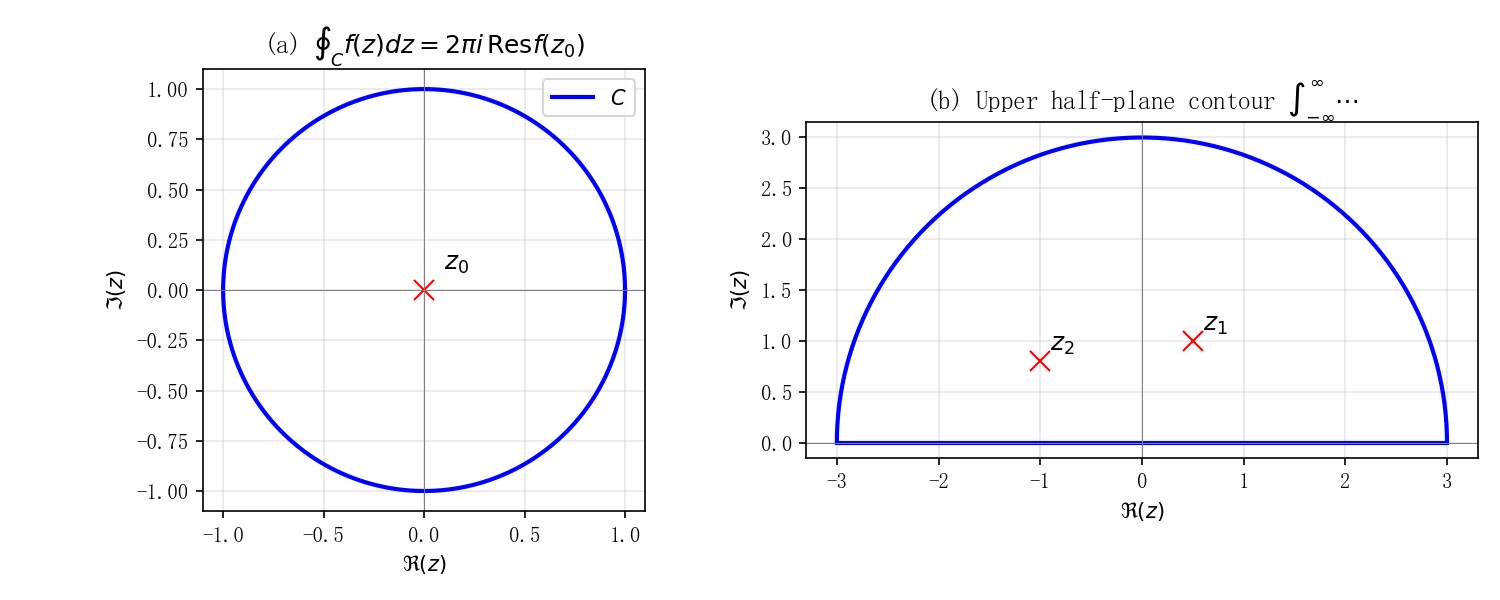
\includegraphics[width=0.75\textwidth]{figures/fig2_2_contour.png}
\caption{左：绕孤立奇点 $z_0$ 的简单围道。右：计算 $\int_{-\infty}^{\infty} f(x)\,\dd x$ 的上半平面围道，$z_1$ 和 $z_2$ 是上半平面的极点。}
\label{fig:contour}
\end{figure}

\subsection{孤立奇点的分类}

\textbf{可去奇点：} $\lim_{z\to z_0}f(z)$ 存在有限。例如 $z=0$ 是 $\sin z/z$ 的可去奇点（因为极限为 $1$）。通过重新定义 $f(0)=1$，奇点可以被"消除"。

\textbf{极点：} $\lim_{z\to z_0}|f(z)| = \infty$。$n$ 阶极点意味着 $(z-z_0)^n f(z)$ 在 $z_0$ 解析且非零。例如 $f(z)=1/(z-1)^2$ 在 $z=1$ 处有二阶极点。

\textbf{本性奇点：} 极限不存在也不为无穷。例如 $z=0$ 是 $e^{1/z}$ 的本性奇点。在本性奇点的任意邻域内，函数可以取到任意复值（Casorati-Weierstrass 定理）。

\begin{example}[奇点分类练习]
对下列函数分类其奇点：

\textbf{(1)} $f(z) = \frac{z}{(z-1)(z+2)}$：$z=1$ 和 $z=-2$ 都是一阶极点。

\textbf{(2)} $f(z) = \frac{\sin z}{z^3}$：$z=0$。展开 $\sin z = z - z^3/3! + z^5/5! - \cdots$，所以 $f(z) = 1/z^2 - 1/6 + \cdots$，这是一个二阶极点。

\textbf{(3)} $f(z) = e^{1/z}$：$z=0$ 是本性奇点。洛朗展开为 $\sum_{n=0}^{\infty} 1/(n! z^n)$，负幂项无限多。

\textbf{(4)} $f(z) = \frac{z^2-1}{z-1}$：化简为 $z+1$（$z\neq1$），所以 $z=1$ 是可去奇点。
\end{example}

\subsection{洛朗展开}

在奇点 $z_0$ 附近，$f(z)$ 可以展开为洛朗级数：
\begin{equation}
f(z) = \sum_{n=-\infty}^{\infty} a_n (z-z_0)^n,
\end{equation}
其中
\begin{equation}
a_n = \frac{1}{2\pi\mathrm{i}}\oint_C \frac{f(z)}{(z-z_0)^{n+1}}\,\dd z.
\end{equation}

洛朗级数是泰勒级数的推广——它允许负幂项的存在。负幂项的存在与否直接对应奇点的类型：
\begin{itemize}
\item 无负幂项 $\to$ 可去奇点（实际上就是泰勒级数）。
\item 有限多项负幂 $\to$ 极点（最高负幂指数 $m$ 就是极点的阶）。
\item 无限多项负幂 $\to$ 本性奇点。
\end{itemize}

\textbf{留数} 就是 $a_{-1}$，即 $(z-z_0)^{-1}$ 项的系数：
\begin{equation}
\mathop{\mathrm{Res}}_{z=z_0} f(z) = a_{-1}
= \frac{1}{2\pi\mathrm{i}}\oint_{C_0} f(z)\,\dd z.
\label{eq:residue_def}
\end{equation}

\textbf{极点留数的计算：} 对于一阶极点，
\begin{equation}
\mathop{\mathrm{Res}}_{z=z_0} f(z) = \lim_{z\to z_0} (z-z_0)f(z).
\end{equation}
对于 $m$ 阶极点，
\begin{equation}
\mathop{\mathrm{Res}}_{z=z_0} f(z)
= \frac{1}{(m-1)!}\lim_{z\to z_0}
\frac{\dd^{m-1}}{\dd z^{m-1}}\left[(z-z_0)^m f(z)\right].
\label{eq:residue_pole}
\end{equation}

\begin{example}[留数计算练习]
计算下列函数在指定点的留数。

\textbf{(1)} $f(z) = \frac{1}{z-1}$，$z_0=1$：一阶极点。
$\mathop{\mathrm{Res}}_{z=1} f(z) = \lim_{z\to 1} (z-1)\frac{1}{z-1} = 1$。

\textbf{(2)} $f(z) = \frac{1}{(z-1)^2}$，$z_0=1$：二阶极点。
由公式：$\mathop{\mathrm{Res}}_{z=1}\frac{1}{(z-1)^2} = \frac{1}{1!}\lim_{z\to1}\frac{\dd}{\dd z}\left[(z-1)^2\frac{1}{(z-1)^2}\right] = \lim_{z\to1}\frac{\dd}{\dd z}(1)=0$。
直接观察洛朗展开：$f(z) = (z-1)^{-2}$，没有 $(z-1)^{-1}$ 项，所以留数确实为 $0$。

\textbf{(3)} $f(z) = \frac{e^z}{z^2}$，$z_0=0$：二阶极点。
展开 $e^z = 1 + z + z^2/2 + \cdots$，所以 $f(z) = 1/z^2 + 1/z + 1/2 + \cdots$，留数为 $1$（$z^{-1}$ 的系数）。
用公式验证：$\mathop{\mathrm{Res}}_{z=0}\frac{e^z}{z^2} = \frac{1}{1!}\lim_{z\to0}\frac{\dd}{\dd z}(e^z) = e^0 = 1$。

\textbf{(4)} $f(z) = \frac{1}{z^2+1}$，$z_0=\mathrm{i}$：一阶极点。
$\mathop{\mathrm{Res}}_{z=\mathrm{i}}\frac{1}{z^2+1} = \lim_{z\to\mathrm{i}} (z-\mathrm{i})\frac{1}{(z-\mathrm{i})(z+\mathrm{i})} = \frac{1}{2\mathrm{i}}$。
\end{example}

\subsection{留数定理}

\textbf{留数定理：} 设 $f(z)$ 在简单闭曲线 $C$ 内部除有限个孤立奇点 $z_1,\dots,z_n$ 外处处解析，在 $C$ 上解析，则
\begin{equation}
\boxed{\;\oint_C f(z)\,\dd z = 2\pi\mathrm{i}\sum_{k=1}^n
\mathop{\mathrm{Res}}_{z=z_k} f(z)\;}.
\label{eq:residue_theorem}
\end{equation}

这是复变函数论中最强大的定理——它将围道积分化为留数求和。

\subsection{实积分的计算}

留数定理最重要的应用之一是计算各种类型的实积分。我们按类型逐一讨论。

\subsubsection{类型 I：$\int_{-\infty}^{\infty} R(x)\,\dd x$，$R(x)$ 是有理函数}

要求 $R(x)$ 的分母次数至少比分子次数高 2 次，且分母无实零点。

\begin{example}[完整算例：$\displaystyle\int_{-\infty}^{\infty} \frac{\dd x}{1+x^2}$]
\textbf{步骤 1：构造复变函数。}
$f(z) = \frac{1}{1+z^2} = \frac{1}{(z+\mathrm{i})(z-\mathrm{i})}$。
$f(z)$ 有奇点 $z=\pm\mathrm{i}$。

\textbf{步骤 2：选择围道。}
取上半平面的半圆围道 $C_R = [-R,R] \cup \Gamma_R$（$\Gamma_R$ 是半径为 $R$ 的上半圆）。
当 $R\to\infty$ 时，$\Gamma_R$ 上的积分趋于零（因为 $|f(z)|\sim 1/R^2$，由 ML 不等式知 $|\int_{\Gamma_R}| \leq \pi R / R^2 = \pi/R \to 0$）。

\textbf{步骤 3：确定围道内的奇点。}
上半平面内的奇点只有 $z=\mathrm{i}$（一阶极点）。

\textbf{步骤 4：计算留数。}
\begin{equation}
\mathop{\mathrm{Res}}_{z=\mathrm{i}} \frac{1}{1+z^2}
= \lim_{z\to\mathrm{i}} (z-\mathrm{i})\frac{1}{(z-\mathrm{i})(z+\mathrm{i})}
= \frac{1}{\mathrm{i}+\mathrm{i}} = \frac{1}{2\mathrm{i}}.
\end{equation}

\textbf{步骤 5：应用留数定理。}
\begin{align*}
\oint_{C_R} f(z)\,\dd z
&= \int_{-R}^{R} \frac{\dd x}{1+x^2} + \int_{\Gamma_R} \frac{\dd z}{1+z^2} \\
&= 2\pi\mathrm{i} \cdot \frac{1}{2\mathrm{i}} = \pi.
\end{align*}
取 $R\to\infty$：
\begin{equation}
\int_{-\infty}^{\infty} \frac{\dd x}{1+x^2} = \pi.
\end{equation}
\textbf{结果印证：} $\arctan x|_{-\infty}^{\infty} = \pi/2 - (-\pi/2) = \pi$。一致！
\end{example}

\subsubsection{类型 II：$\int_{-\infty}^{\infty} R(x) e^{\mathrm{i}ax}\,\dd x$（含三角函数的积分）}

对这类积分，Jordan 引理提供了半圆上积分趋于零的条件。

\textbf{Jordan 引理：} 若 $f(z)$ 在上半平面当 $|z|\to\infty$ 时一致趋于 $0$，则对 $a>0$，
\begin{equation}
\lim_{R\to\infty}\int_{\Gamma_R} f(z) e^{\mathrm{i}az}\,\dd z = 0,
\end{equation}
其中 $\Gamma_R$ 是上半圆 $|z|=R$, $\Im z \geq 0$。

\begin{example}[完整算例：$\displaystyle\int_{-\infty}^{\infty} \frac{\cos x}{x^2+1}\,\dd x$]
\textbf{步骤 1：构造复变函数。}
考虑 $\displaystyle I = \int_{-\infty}^{\infty} \frac{e^{\mathrm{i}x}}{x^2+1}\,\dd x$，
目标积分为 $\Re(I)$。

令 $f(z) = \frac{e^{\mathrm{i}z}}{z^2+1}$。

\textbf{步骤 2：围道和奇点。}
上半平面半圆围道。奇点 $z=\pm\mathrm{i}$。上半平面内只有 $z=\mathrm{i}$。

\textbf{步骤 3：计算留数（一阶极点）。}
\begin{align*}
\mathop{\mathrm{Res}}_{z=\mathrm{i}} \frac{e^{\mathrm{i}z}}{(z+\mathrm{i})(z-\mathrm{i})}
&= \lim_{z\to\mathrm{i}} (z-\mathrm{i})\frac{e^{\mathrm{i}z}}{(z+\mathrm{i})(z-\mathrm{i})}
= \frac{e^{\mathrm{i}\cdot\mathrm{i}}}{\mathrm{i}+\mathrm{i}}
= \frac{e^{-1}}{2\mathrm{i}}.
\end{align*}

\textbf{步骤 4：应用留数定理。}
由 Jordan 引理，半圆上的积分在 $R\to\infty$ 时为零。因此
\begin{equation}
I = \int_{-\infty}^{\infty} \frac{e^{\mathrm{i}x}}{x^2+1}\,\dd x
= 2\pi\mathrm{i} \cdot \frac{e^{-1}}{2\mathrm{i}} = \frac{\pi}{e}.
\end{equation}

\textbf{步骤 5：取实部。}
\begin{equation}
\boxed{\;\int_{-\infty}^{\infty} \frac{\cos x}{x^2+1}\,\dd x = \frac{\pi}{e}\;},
\qquad
\int_{-\infty}^{\infty} \frac{\sin x}{x^2+1}\,\dd x = 0 \text{（奇函数）}.
\end{equation}
\end{example}

\begin{example}[$\displaystyle\int_0^{\infty} \frac{\sin x}{x}\,\dd x = \frac{\pi}{2}$]
这是物理学中最重要的积分之一，出现在衍射理论、信号处理和量子力学中。

\textbf{构造：} 考虑 $f(z) = \frac{e^{\mathrm{i}z}}{z}$，并取如下围道：由实轴 $[-R,-\varepsilon]$、小半圆 $C_\varepsilon$（半径 $\varepsilon$，上半平面）、实轴 $[\varepsilon,R]$、大半圆 $\Gamma_R$（半径 $R$）组成。

由于 $\frac{e^{\mathrm{i}z}}{z}$ 在围道内解析（原点被小半圆避开），总积分为 $0$：
\begin{equation}
\int_{-R}^{-\varepsilon} \frac{e^{\mathrm{i}x}}{x}\,\dd x
+ \int_{C_\varepsilon} \frac{e^{\mathrm{i}z}}{z}\,\dd z
+ \int_{\varepsilon}^{R} \frac{e^{\mathrm{i}x}}{x}\,\dd x
+ \int_{\Gamma_R} \frac{e^{\mathrm{i}z}}{z}\,\dd z = 0.
\end{equation}

$R\to\infty$ 时，$\Gamma_R$ 上积分由 Jordan 引理趋于 $0$。
$\varepsilon\to0$ 时，小半圆上的积分 $= -\pi\mathrm{i}\,\mathop{\mathrm{Res}}_{z=0}\frac{e^{\mathrm{i}z}}{z} = -\pi\mathrm{i}\cdot 1 = -\pi\mathrm{i}$（负号因为顺时针方向）。

合并实轴上的积分：
\begin{equation}
\int_{-\infty}^{\infty} \frac{e^{\mathrm{i}x}}{x}\,\dd x = \pi\mathrm{i}.
\end{equation}

取虚部：
\begin{equation}
\int_{-\infty}^{\infty} \frac{\sin x}{x}\,\dd x = \pi,\quad
\int_{0}^{\infty} \frac{\sin x}{x}\,\dd x = \frac{\pi}{2}.
\end{equation}
\end{example}

\subsubsection{类型 III：$\int_0^{2\pi} R(\cos\theta,\sin\theta)\,\dd\theta$}

令 $z = e^{\mathrm{i}\theta}$，则 $\cos\theta = (z+z^{-1})/2$，$\sin\theta = (z-z^{-1})/(2\mathrm{i})$，$\dd\theta = \dd z/(\mathrm{i}z)$：
\begin{equation}
\int_0^{2\pi} R(\cos\theta,\sin\theta)\,\dd\theta
= \oint_{|z|=1} \frac{1}{\mathrm{i}z}R\left(\frac{z+z^{-1}}{2},
\frac{z-z^{-1}}{2\mathrm{i}}\right)\dd z.
\end{equation}

\begin{example}[$\displaystyle\int_0^{2\pi} \frac{\dd\theta}{a+\cos\theta}$, $a>1$]
令 $z=e^{\mathrm{i}\theta}$，$\cos\theta = (z+z^{-1})/2$，$\dd\theta = \dd z/(\mathrm{i}z)$：
\begin{align*}
I &= \oint_{|z|=1} \frac{1}{\mathrm{i}z}\frac{1}{a + (z+z^{-1})/2}\,\dd z
= \oint_{|z|=1} \frac{2}{\mathrm{i}(2az + z^2 + 1)}\,\dd z \\
&= \frac{2}{\mathrm{i}}\oint_{|z|=1} \frac{1}{z^2 + 2az + 1}\,\dd z.
\end{align*}

分母的根为 $z = -a \pm \sqrt{a^2-1}$。由于 $a>1$，$z_1 = -a + \sqrt{a^2-1}$ 在单位圆内，$z_2 = -a - \sqrt{a^2-1}$ 在单位圆外。

$z_1$ 处是一阶极点，留数为：
\begin{align*}
\mathop{\mathrm{Res}}_{z=z_1} \frac{1}{z^2+2az+1}
&= \lim_{z\to z_1} \frac{z-z_1}{(z-z_1)(z-z_2)} = \frac{1}{z_1 - z_2} \\
&= \frac{1}{2\sqrt{a^2-1}}.
\end{align*}

由留数定理：
\begin{equation}
I = \frac{2}{\mathrm{i}} \cdot 2\pi\mathrm{i} \cdot \frac{1}{2\sqrt{a^2-1}}
= \frac{2\pi}{\sqrt{a^2-1}}.
\end{equation}

验证：当 $a\to\infty$ 时 $I\to0$，符合直觉（分母很大，积分趋近于 0）。
\end{example}

\subsubsection{类型 IV：含支点的积分}

当被积函数含有多值函数（如 $\sqrt{z}$, $\ln z$）时，需要引入割线围道。

\begin{example}[$\displaystyle\int_0^{\infty} \frac{\sqrt{x}}{1+x^2}\,\dd x$]
\textbf{构造：} 考虑 $f(z) = \frac{\sqrt{z}}{1+z^2}$，其中取 $\sqrt{z}$ 的主值分支（割线沿正实轴）。

围道选择：从 $\varepsilon$ 到 $R$ 的上岸（$\arg z = 0$），大半圆 $\Gamma_R$，从 $R$ 到 $\varepsilon$ 的下岸（$\arg z = 2\pi$），以及小圆 $C_\varepsilon$。

在上岸：$\sqrt{z} = \sqrt{x}$；在下岸：$\sqrt{z} = \sqrt{x}e^{\mathrm{i}\pi} = -\sqrt{x}$。

围道内的奇点：$z=\mathrm{i}$ 和 $z=-\mathrm{i}$，留数分别为：
\begin{align*}
\mathop{\mathrm{Res}}_{z=\mathrm{i}} \frac{\sqrt{z}}{1+z^2} &= \frac{\sqrt{\mathrm{i}}}{2\mathrm{i}} = \frac{e^{\mathrm{i}\pi/4}}{2\mathrm{i}},\\
\mathop{\mathrm{Res}}_{z=-\mathrm{i}} \frac{\sqrt{z}}{1+z^2} &= \frac{\sqrt{-\mathrm{i}}}{-2\mathrm{i}} = \frac{e^{-\mathrm{i}\pi/4}}{-2\mathrm{i}}.
\end{align*}

留数之和：
\[
\frac{e^{\mathrm{i}\pi/4}}{2\mathrm{i}} - \frac{e^{-\mathrm{i}\pi/4}}{2\mathrm{i}} = \frac{1}{\mathrm{i}}\sin\frac{\pi}{4} = \frac{1}{\sqrt{2}\mathrm{i}}.
\]

围道积分为 $2\pi\mathrm{i} \cdot \frac{1}{\sqrt{2}\mathrm{i}} = \sqrt{2}\pi$。

另一方面，上岸积分 $+$ 下岸积分 $= \int_0^{\infty} \frac{\sqrt{x}}{1+x^2}\,\dd x + \int_{\infty}^{0} \frac{-\sqrt{x}}{1+x^2}\,\dd x = 2\int_0^{\infty} \frac{\sqrt{x}}{1+x^2}\,\dd x$。

大半圆和小圆上的积分在 $R\to\infty$, $\varepsilon\to0$ 时趋于零。

因此：
\begin{equation}
\int_0^{\infty} \frac{\sqrt{x}}{1+x^2}\,\dd x = \frac{\sqrt{2}\pi}{2} = \frac{\pi}{\sqrt{2}}.
\end{equation}
\end{example}

\begin{insight}[量子散射理论中的留数]
在量子力学中，散射振幅 $f(\theta)$ 作为复能量 $E$ 的函数在复平面上有极点结构。\textbf{极点对应束缚态}（实轴下方的极点对应共振态），而\textbf{割线对应连续谱阈值}。留数定理在这里揭示了散射的解析结构与能谱之间的深刻联系——这正是 $S$ 矩阵理论的核心思想。
\end{insight}

\subsection{围道积分技巧总结}

\begin{table}[h]
\centering
\caption{常见围道积分类型与策略}
\label{tab:contour_types}
\begin{tabular}{c|c|c}
\toprule
积分类型 & 典型形式 & 围道策略 \\
\midrule
I & $\int_{-\infty}^{\infty} R(x)\,\dd x$ & 上半/下半平面半圆 + ML 引理 \\
II & $\int_{-\infty}^{\infty} R(x)\sin(ax)\,\dd x$ & 半圆 + Jordan 引理，取虚部 \\
III & $\int_0^{2\pi} R(\cos\theta,\sin\theta)\,\dd\theta$ & 单位圆 $z = e^{\mathrm{i}\theta}$ \\
IV & $\int_0^{\infty} x^{\alpha-1} R(x)\,\dd x$ & 割线围道（Keyhole contour） \\
V & $\int_{-\infty}^{\infty} \frac{f(x)}{x-x_0}\,\dd x$ & 主值积分 + 小半圆绕过奇点 \\
\bottomrule
\end{tabular}
\end{table}

\section{保角映射与二维场问题}
\label{sec:conformal}

\subsection*{动机：如何把复杂边界变成简单边界？}

两个平行板间的电场可以解析求解。但如果一个板是弯曲的，或者带尖角？\textbf{保角映射} 把一个具有复杂几何边界的物理区域映射到一个已经知道解的标准区域。你只需把已知解"拉回"到原来的坐标系。

\subsection{保角性}

解析函数 $w = f(z)$ 在 $f'(z)\neq0$ 的点处具有保角性：两条曲线之间的夹角在映射下保持不变。

\textbf{几何意义：} 解析映射是局部的旋转和缩放变换。$|f'(z)|$ 是局部缩放因子，$\arg f'(z)$ 是局部旋转角。

% 保角映射示意图
\begin{figure}[H]
\centering
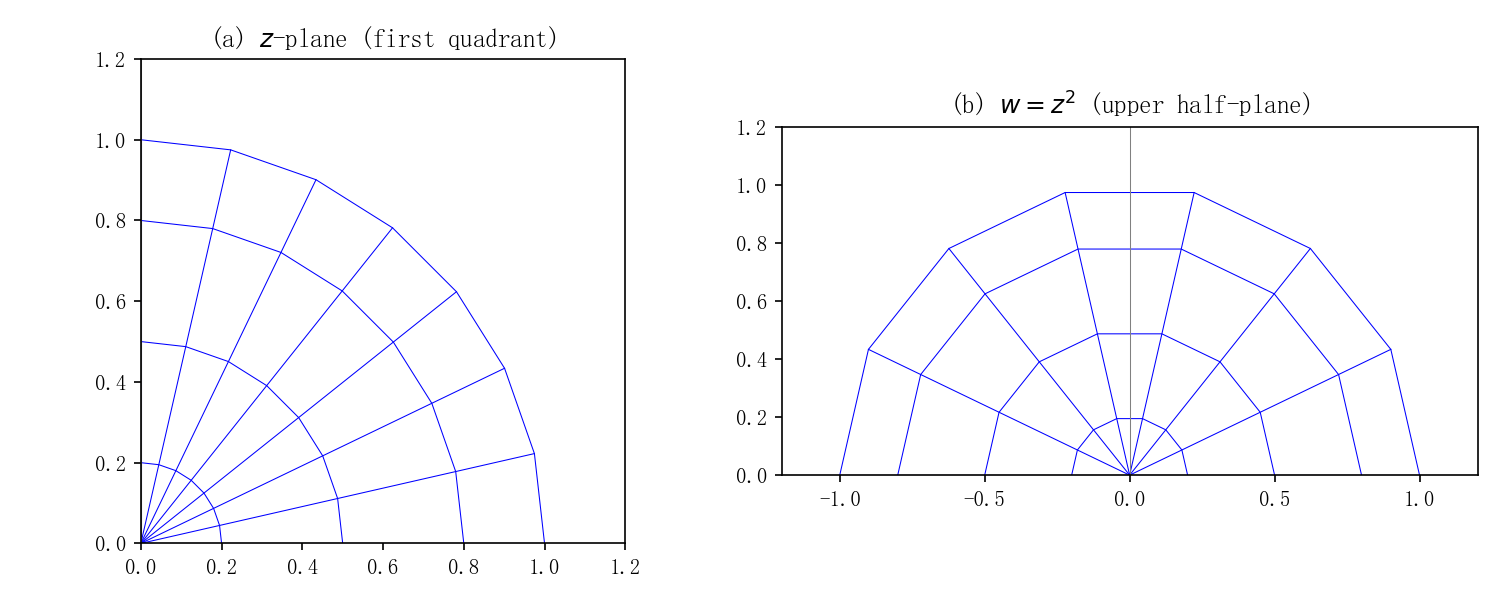
\includegraphics[width=0.75\textwidth]{figures/fig2_3_conformal.png}
\caption{$w=z^2$ 的保角映射：(a) $z$ 平面上的第一象限扇形；(b) 映射后的上半平面 $w$ 平面。注意原先在原点相交于 $90^\circ$ 的边界线变成了 $180^\circ$——因为 $f'(0)=0$，保角性在 $f'(z)=0$ 处失效。}
\label{fig:conformal}
\end{figure}

\subsection{基本映射}

\begin{itemize}
\item $w = z + a$：平移
\item $w = e^{\mathrm{i}\alpha}z$：旋转 $\alpha$
\item $w = kz$：缩放
\item $w = 1/z$：反演（将圆变为圆或直线）
\item $w = z^2$：将角域映射为上半平面
\item $w = \sqrt{z}$：将角域映射为半平面（$z^2$ 的逆映射）
\item $w = e^z$：将水平带形映射为角域
\item $w = \ln z$：将角域映射为带形（$e^z$ 的逆映射）
\end{itemize}

\begin{example}[用保角映射求解静电场]
设有两个半无限平行板电极，电势分别为 $\phi=0$ 和 $\phi=V$，间距 $d$。
映射 $w = e^{\pi z/d}$ 将带形区域 $0<\Im z<d$ 映射为上半平面 $\Im w>0$，而平行板电容器中均匀场的复势 $F(w) = V/\pi\ln w$。最终得到物理平面上的电势分布：
\begin{equation}
\phi(x,y) = \frac{V}{d}\,y,
\qquad
\psi(x,y) = \frac{V}{d}\,x.
\end{equation}
这正是平板电容器的均匀场解。保角映射将复杂边界问题化为标准区域上的已知解。
\end{example}

\subsection{Joukowski 映射与机翼理论}

\textbf{Joukowski 映射：}
\begin{equation}
w = z + \frac{1}{z}.
\label{eq:joukowski}
\end{equation}

这个映射在空气动力学中至关重要——它将圆映射为机翼形状（Joukowski 翼型）。

当 $z = e^{\mathrm{i}\theta}$（单位圆）时，$w = 2\cos\theta$，是实轴上的线段 $[-2,2]$——单位圆被映射为平板。

当 $z = Re^{\mathrm{i}\theta}$（$R>1$，更大的圆）时：
\begin{equation}
w = Re^{\mathrm{i}\theta} + \frac{1}{R}e^{-\mathrm{i}\theta}
= \left(R + \frac{1}{R}\right)\cos\theta + \mathrm{i}\left(R - \frac{1}{R}\right)\sin\theta.
\end{equation}
这是一个椭圆。如果圆心不在原点而在 $(-\varepsilon,0)$，映射得到的曲线就变成了一个具有圆头尖尾的翼型。

\textbf{物理意义：} 绕圆柱的势流解是已知的（复势 $F(z) = U(z + a^2/z)$），通过 Joukowski 映射可以将其变换为绕翼型的流动。这就是\textbf{薄翼理论}的数学基础。

\begin{insight}[保角映射的物理哲学]
保角映射之所以有效，是因为拉普拉斯方程 $\nabla^2\phi=0$ 在解析变换下形式不变。换句话说，\textbf{静电场、稳态热传导、无旋流场、静磁场（无源区）都共享同一数学结构}。当你解出了其中一个问题的保角映射解，就免费得到了所有其他问题的解。这种数学统一性正是物理学家追求的境界。
\end{insight}

\subsection{Schwarz-Christoffel 映射}

\textbf{Schwarz-Christoffel 映射}将上半平面映射到任意多边形内部：
\begin{equation}
w = A\int_{z_0}^{z} (\zeta - x_1)^{\alpha_1-1}(\zeta - x_2)^{\alpha_2-1}\cdots(\zeta - x_n)^{\alpha_n-1}\,\dd\zeta + B,
\label{eq:sc_mapping}
\end{equation}
其中 $\alpha_k\pi$ 是多边形在顶点 $w_k$ 处的内角，$x_k$ 是实轴上对应顶点的原像点。

\begin{example}[直角区域的映射]
考虑映射 $w = \sqrt{z}$。它将上半平面映射为第一象限（一个 $90^\circ$ 角域）。这是 Schwarz-Christoffel 映射在 $n=2$ 时的特例——两个顶点分别在 $0$ 和无穷远，内角均为 $\pi/2$。

在静电学中，这个映射用来求解导体尖角附近的电场分布——尖角处的场强会发散（尖端放电效应），这正是 $\sqrt{z}$ 在 $z=0$ 处导数无穷大的物理表现。
\end{example}

\section{解析函数的物理应用专题}
\label{sec:physics_applications}

\subsection{二维拉普拉斯场的复势}

二维静电场和不可压缩无旋流场可以用复势统一描述。设 $\phi$ 为势函数，$\psi$ 为流函数：
\begin{equation}
F(z) = \phi(x,y) + \mathrm{i}\psi(x,y),\quad
F'(z) = E_x - \mathrm{i}E_y \quad(\text{电场情形}).
\end{equation}

\textbf{物理量对应关系：}
\begin{itemize}
\item $\phi$ = 电势 / 速度势
\item $\psi$ = 流函数（$\nabla\psi$ 旋转 $90^\circ$ 给出场方向）
\item $F'(z)$ = 共轭场强 / 复速度
\end{itemize}

\begin{example}[点源的复势]
位于原点的二维点源（强度 $\lambda$）的复势为：
\begin{equation}
F(z) = \frac{\lambda}{2\pi}\ln z
= \frac{\lambda}{2\pi}(\ln r + \mathrm{i}\theta).
\end{equation}
实部 $\phi = \lambda/(2\pi)\ln r$ 是二维泊松方程的解，对应于无限长线电荷的电势。虚部 $\theta$ 是流函数——流线从原点径向发出。
\end{example}

\begin{example}[电偶极子的复势]
位于 $\pm d/2$ 的一对点源和点汇（强度分别为 $\pm\lambda$）构成偶极子。当 $d\to0$ 时保持 $\lambda d = p$ 有限，复势为：
\begin{equation}
F(z) = \frac{p}{2\pi z}.
\end{equation}
这是二维电偶极子的复势。对应的电场 $E_x - \mathrm{i}E_y = F'(z) = -\frac{p}{2\pi z^2}$。等势线 $\Re(F) = \text{常数}$ 是一族通过原点的圆。
\end{example}

\begin{example}[均匀流绕圆柱]
在均匀流 $U$ 中放置半径为 $a$ 的圆柱，复势为：
\begin{equation}
F(z) = U\left(z + \frac{a^2}{z}\right).
\end{equation}
验证：大 $|z|$ 时 $F(z) \sim Uz$（均匀流），在 $|z|=a$ 处 $\Im(F) = U(r - a^2/r)\sin\theta = 0$，即圆柱表面是一条流线。
\end{example}

\subsection{色散关系与 Kramers-Kronig 关系}

\textbf{因果律 + 解析性 = 色散关系。} 这是复变函数在物理中最深刻的应用之一。

设 $\chi(\omega) = \chi'(\omega) + \mathrm{i}\chi''(\omega)$ 为线性响应函数的频域表示（如介电函数、磁导率、电导率）。因果性要求 $\chi(t)=0$ 对 $t<0$，这导致 $\chi(\omega)$ 在上半复 $\omega$ 平面解析。

对上半平面应用柯西积分公式，取实部和虚部即得 Kramers-Kronig 关系：
\begin{align}
\chi'(\omega) &= \frac{1}{\pi}\mathcal{P}\int_{-\infty}^{\infty}
\frac{\chi''(\omega')}{\omega' - \omega}\,\dd\omega',\\
\chi''(\omega) &= -\frac{1}{\pi}\mathcal{P}\int_{-\infty}^{\infty}
\frac{\chi'(\omega')}{\omega' - \omega}\,\dd\omega'.
\label{eq:kk_relations}
\end{align}

\begin{example}[洛伦兹振子模型]
对于洛伦兹振子模型（经典色散理论），介电函数为：
\begin{equation}
\varepsilon(\omega) = 1 + \frac{\omega_p^2}{\omega_0^2 - \omega^2 - \mathrm{i}\gamma\omega}.
\end{equation}

实部和虚部分别为：
\begin{align}
\varepsilon'(\omega) &= 1 + \frac{\omega_p^2(\omega_0^2 - \omega^2)}{(\omega_0^2 - \omega^2)^2 + \gamma^2\omega^2},\\
\varepsilon''(\omega) &= \frac{\omega_p^2\gamma\omega}{(\omega_0^2 - \omega^2)^2 + \gamma^2\omega^2}.
\end{align}

可以验证这对 $(\varepsilon',\varepsilon'')$ 满足 Kramers-Kronig 关系。在共振频率 $\omega_0$ 附近，$\varepsilon''$ 出现峰值（吸收），而 $\varepsilon'$ 急剧变化（反常色散）。
\end{example}

\begin{insight}
Kramers-Kronig 关系的物理意义振聋发聩：\textbf{如果只知道某个频率下材料的吸收谱（$\chi''$ 的虚部），就可以唯一地计算出色散（$\chi'$ 的实部）}。反之亦然。这意味着"吸收"和"色散"不是独立的物质性质——它们是同一个解析函数在实轴上的实部和虚部。光学中折射率和消光系数的关系、粒子物理中 forward scattering 的色散关系，都源于此。
\end{insight}

\subsection{线性系统的传递函数与解析性}

在线性系统理论中，传递函数 $H(s)$ 是 $s$ 的复变函数。系统的因果性等价于 $H(s)$ 的收敛域（ROC）是某个右半平面。稳定性等价于 $H(s)$ 的所有极点具有负实部（即位于左半平面）。

\begin{example}[RC 低通滤波器的传递函数]
\begin{equation}
H(s) = \frac{1}{1 + sRC},\quad \Re(s) > -\frac{1}{RC}.
\end{equation}
极点在 $s = -1/(RC)$（左半平面），因此系统稳定。单位冲激响应为：
\begin{equation}
h(t) = \frac{1}{RC}e^{-t/(RC)}\Theta(t).
\end{equation}
验证因果性：$t<0$ 时 $h(t)=0$。
\end{example}

\subsection{傅里叶变换与解析延拓}

拉普拉斯变换 $F(s)$ 是傅里叶变换 $\tilde{f}(\omega)$ 的解析延拓：
\begin{equation}
F(\sigma + \mathrm{i}\omega) = \int_0^{\infty} f(t) e^{-\sigma t} e^{-\mathrm{i}\omega t}\,\dd t.
\end{equation}

当 $\sigma=0$ 时退化为傅里叶变换（如果收敛）。这个联系表明：\textbf{拉普拉斯变换 = 傅里叶变换 + 收敛因子}。这正是第 3 章的核心内容之一。

\section{本章小结}

\begin{itemize}
\item \textbf{复数与相量法} 将时域微积分化为频域代数，是线性系统分析的利器。
\item \textbf{柯西-黎曼方程} 是解析函数的定义性特征，它将解析函数与二维拉普拉斯场紧密联系。
\item \textbf{柯西积分定理与公式} 表明解析函数具有"边界决定内部"的刚性。
\item \textbf{留数定理} 将围道积分化为留数求和，是计算实积分和反常积分的标准工具。
\item \textbf{保角映射} 将复杂几何边界的物理问题映射到标准区域求解。
\item \textbf{解析性与因果性} 的结合导出 Kramers-Kronig 关系，是所有线性响应系统的普适约束。
\end{itemize}

\subsection*{概念图谱}

\begin{center}
\fbox{\parbox{0.92\textwidth}{
\textbf{复变函数的概念网络：}\\[3pt]
$\bullet$ 复数代数 $\to$ 相量法（交流电路）\\[3pt]
$\bullet$ 柯西-黎曼方程 $\to$ 调和函数 $\to$ 二维场（静电/流体）$\to$ 复势 \\[3pt]
$\bullet$ 柯西积分定理 $\to$ 柯西积分公式 $\to$ 高阶导数公式 $\to$ 泊松积分公式\\[3pt]
$\bullet$ 洛朗展开 $\to$ 留数 $\to$ 留数定理 $\to$ 实积分计算 / Kramers-Kronig 关系\\[3pt]
$\bullet$ 解析函数 $\to$ 保角映射 $\to$ 二维边值问题统一解法\\[3pt]
$\bullet$ 多值函数 $\to$ 黎曼曲面 $\to$ 割线围道积分
}}
\end{center}

\subsection*{公式参考表}

\begin{table}[h]
\centering
\caption{复变函数核心公式速查}
\label{tab:complex_formulas}
\begin{tabular}{c|c}
\toprule
公式 & 说明 \\
\midrule
$e^{\mathrm{i}\theta} = \cos\theta + \mathrm{i}\sin\theta$ & 欧拉公式 \\
$\frac{\partial u}{\partial x} = \frac{\partial v}{\partial y},\; \frac{\partial u}{\partial y} = -\frac{\partial v}{\partial x}$ & 柯西-黎曼方程 \\
$\oint_C f(z)\,\dd z = 0$（$f$ 在 $C$ 内解析） & 柯西积分定理 \\
$f(z_0) = \frac{1}{2\pi\mathrm{i}}\oint_C \frac{f(z)}{z-z_0}\,\dd z$ & 柯西积分公式 \\
$f^{(n)}(z_0) = \frac{n!}{2\pi\mathrm{i}}\oint_C \frac{f(z)}{(z-z_0)^{n+1}}\,\dd z$ & 高阶导数公式 \\
$\oint_C f(z)\,\dd z = 2\pi\mathrm{i}\sum\mathop{\mathrm{Res}} f(z_k)$ & 留数定理 \\
$\mathop{\mathrm{Res}}_{z=z_0} f = \lim_{z\to z_0}(z-z_0)f(z)$ & 一阶极点留数 \\
$\mathop{\mathrm{Res}}_{z=z_0} f = \frac{1}{(m-1)!}\lim_{z\to z_0}\frac{d^{m-1}}{dz^{m-1}}[(z-z_0)^m f(z)]$ & $m$ 阶极点留数 \\
$w = z + 1/z$ & Joukowski 映射 \\
$\chi'(\omega) = \frac{1}{\pi}\mathcal{P}\int\frac{\chi''(\omega')}{\omega'-\omega}\,\dd\omega'$ & Kramers-Kronig 关系 \\
\bottomrule
\end{tabular}
\end{table}

\begin{insight}
回顾第 2 章，你会发现一条主线：\textbf{从复数的代数引入 $\to$ 解析函数的微分约束 $\to$ 整体积分性质 $\to$ 留数与奇点结构 $\to$ 物理应用}。这与第 1 章中"局部微分 $\to$ 整体积分"的思维模式一脉相承。在复变函数的语境中，局部就是柯西-黎曼方程，整体就是留数定理。
\end{insight}

\section*{习题}

\textbf{基础题（巩固概念）}

\begin{enumerate}
\item 将复数 $z = 1 + \mathrm{i}\sqrt{3}$ 化为极坐标形式 $re^{\mathrm{i}\theta}$。计算 $z^{10}$。
\item 计算下列复数的实部、虚部、模和辐角主值：
(1) $(1+\mathrm{i})^3$；(2) $\frac{1-\mathrm{i}}{1+\mathrm{i}}$；(3) $e^{2+\mathrm{i}\pi/3}$。
\item 判断下列函数在何处可导，在何处解析：
(1) $f(z) = \bar{z}^2$；(2) $f(z) = e^z$；(3) $f(z) = \Re(z)$；
(4) $f(z) = \sin z$。
\item 验证 $u(x,y) = e^x\cos y$ 是调和函数，并求其共轭调和函数 $v(x,y)$，写出 $f(z)=u+\mathrm{i}v$ 的显式表达式。
\item 计算 $\displaystyle\int_C \frac{\dd z}{z-1}$，$C$ 为 $|z-1|=1$ 的逆时针圆周。
\item 求 $f(z) = \frac{z}{(z-1)(z-2)}$ 在 $z=1$ 和 $z=2$ 处的留数。
\end{enumerate}

\textbf{提高题（应用分析）}

\begin{enumerate}
\item[7.] 利用留数定理计算 $\displaystyle\int_0^{2\pi}\frac{\dd\theta}{a+\cos\theta}$（$a>1$）。写出完整步骤并验证结果的合理性（当 $a\to\infty$ 时积分应趋近于 0）。
\item[8.] 计算 $\displaystyle\int_{-\infty}^{\infty}\frac{x^2}{x^4+1}\,\dd x$。\textbf{提示：} 分母有四个一阶极点 $e^{\mathrm{i}\pi/4}, e^{3\mathrm{i}\pi/4}, e^{5\mathrm{i}\pi/4}, e^{7\mathrm{i}\pi/4}$，只取上半平面的两个。
\item[9.] 求映射 $w = z + 1/z$ 将单位圆 $|z|=1$ 映射为什么曲线？该映射在二维理想流体的圆柱绕流问题中有何应用？\textbf{提示：} $z=e^{\mathrm{i}\theta}$ 时 $w = 2\cos\theta$ 是实轴上的线段。
\item[10.] 计算洛朗展开：在 $z=0$ 附近将 $f(z) = \frac{1}{z(z-1)}$ 展开为洛朗级数。分别在 $0<|z|<1$ 和 $|z|>1$ 两个区域写出展开式。
\item[11.] 求 RC 串联电路（$C=10\mu\text{F}$, $R=1\text{k}\Omega$）的传递函数、截止频率和幅频响应 $|H(\omega)|$ 的表达式。当输入 $V_{\text{in}}(t) = 10\cos(100t)$ 时，求稳态输出。
\item[12.] 计算 $\displaystyle\int_0^{\infty} \frac{\sin x}{x}\,\dd x = \frac{\pi}{2}$ 用 Jordan 引理和围道积分验证。
\end{enumerate}

\textbf{挑战题（综合拓展）}

\begin{enumerate}
\item[13.]（双线性变换）映射 $w = \frac{z-1}{z+1}$ 将右半平面 $\Re(z)>0$ 映射到单位圆 $|w|<1$。证明这一性质。该映射在控制理论中用于将 $s$ 平面的稳定性边界映射到 $z$ 平面的单位圆。
\item[14.]（Kramers-Kronig 练习）设 $\chi''(\omega) = \frac{\omega}{1+\omega^2}$，利用 Kramers-Kronig 关系求 $\chi'(\omega)$。\textbf{提示：} 用留数定理计算主值积分。验证你的结果满足 $\chi(-\omega) = \chi^*(\omega)$（实信号的对称性）。
\item[15.]（量子散射）一维薛定谔方程的一个解为 $\psi(x) \sim e^{\mathrm{i}kx} + f(k)\frac{e^{\mathrm{i}k|x|}}{|x|}$。散射振幅 $f(k)$ 在复 $k$ 平面上有极点 $k=\mathrm{i}\kappa$（$\kappa>0$），证明这对应束缚态，其能量为 $E = -\hbar^2\kappa^2/(2m)$。
\item[16.]（保角映射与传热）一半无限大平板 $x>0$，$y=0$ 边界上温度分布为 $T(x,0)=T_0\Theta(a-|x|)$（即 $|x|<a$ 处 $T=T_0$，其余 $T=0$）。通过适当的保角映射和复势方法，求平板上方的稳态温度分布。
\item[17.]（割线围道积分）计算 $\displaystyle\int_0^{\infty} \frac{\ln x}{1+x^2}\,\dd x$。\textbf{提示：} 考虑 $f(z) = \frac{(\ln z)^2}{1+z^2}$ 的围道积分，取割线沿正实轴。
\item[18.]（Joukowski 翼型）设 $z$ 平面上的圆为 $|z - \varepsilon| = 1 + \varepsilon$（$\varepsilon>0$ 小量），圆心在 $(\varepsilon,0)$。通过 Joukowski 映射 $w = z + 1/z$ 得到翼型形状。证明翼型在 $w=2$ 处有尖点（后缘），并画出 $\varepsilon=0.1$ 时的翼型轮廓。
\end{enumerate}
